%\documentclass[12pt]{article}  % standard LaTeX, 12 point type
\documentclass[sigconf]{acmart}

\usepackage{booktabs} % For formal tables
\usepackage{multirow}
\usepackage{listings}   

\usepackage{amsfonts,latexsym}
\usepackage{amsthm}
\usepackage{amssymb}
\usepackage[utf8x]{inputenc} % Кодировка
\usepackage[english]{babel} % Многоязычность
\usepackage{amsmath}
\usepackage{tikz}
\usetikzlibrary{automata,positioning}
\usetikzlibrary{graphs, graphs.standard, quotes}
\usetikzlibrary{arrows,decorations.pathmorphing,backgrounds,positioning,fit,petri}


\usepackage{algpseudocode}
\usepackage{algorithm}
\usepackage{caption}
\usepackage{algorithmicx}
\usepackage{systeme}



\newtheorem{theorem}{Theorem}[section]
\newtheorem{proposition}[theorem]{Proposition}
\newtheorem{lemma}[theorem]{Lemma}
\newtheorem{corollary}[theorem]{Corollary}
\newtheorem{conjecture}[theorem]{Conjecture}

\theoremstyle{definition}
\newtheorem{definition}{Определение}[section]
\newtheorem{example}{Example}[section]

% unnumbered environments:

\theoremstyle{remark}
\newtheorem*{remark}{Remark}
\newtheorem*{notation}{Notation}
\newtheorem*{note}{Note}

\setlength{\parskip}{5pt plus 2pt minus 1pt}
%\setlength{\parindent}{0pt}

\usepackage{color}
\usepackage{listings}
\usepackage{caption}
\usepackage{graphicx}
\usepackage{ucs}

\setcounter{MaxMatrixCols}{20}


\newcommand{\tab}[1][0.3cm]{\ensuremath{\hspace*{#1}}}
% A generalized view on parsing and translation
% http://dl.acm.org/citation.cfm?id=2206331
\title{Rytter-style Algorithm for Context-Fre Path Querying}

\author{Semyon Grigorev}
\orcid{0000-0002-7966-0698}
\affiliation{%
  \institution{Saint Petersburg State University}
  \streetaddress{7/9 Universitetskaya nab.}
  \city{St. Petersburg}
  \country{Russia}
  \postcode{199034}
}
\email{semen.grigorev@jetbrains.com}


\author{Ekaterina Shemetova}
\affiliation{%
  \institution{Saint Petersburg State University}
  \streetaddress{7/9 Universitetskaya nab.}
  \city{St. Petersburg}
  \country{Russia}
  \postcode{199034}
}
\email{katyacyfra@gmail.com}




\date{\today}

\textwidth=190mm
\textheight=250mm
\topmargin=-20mm
\oddsidemargin=-15mm
\evensidemargin=-15mm


\begin{document}

\algtext*{EndWhile}% Remove "end while" text
\algtext*{EndIf}% Remove "end if" text
\algtext*{EndFor}% Remove "end for" text
\algtext*{EndFunction}% Remove "end function" text


%\begin{abstract}
%Abstract
%\end{abstract}

%
% The code below should be generated by the tool at
% http://dl.acm.org/ccs.cfm
% Please copy and paste the code instead of the example below.
%
%\begin{CCSXML}
%<ccs2012>
%<concept>
%<concept_id>10002951.10002952.10002953.10010146</concept_id>
%<concept_desc>Information systems~Graph-based database models</concept_desc>
%<concept_significance>500</concept_significance>
%</concept>
%<concept>
%<concept_id>10002951.10002952.10003197.10010825</concept_id>
%<concept_desc>Information systems~Query languages for non-relational engines</concept_desc>
%<concept_significance>500</concept_significance>
%</concept>
%<concept>
%<concept_id>10011007.10011006.10011008.10011009.10011012</concept_id>
%<concept_desc>Software and its engineering~Functional languages</concept_desc>
%<concept_significance>300</concept_significance>
%</concept>
%<concept>
%<concept_id>10003752.10003766.10003771</concept_id>
%<concept_desc>Theory of computation~Grammars and context-free languages</concept_desc>
%<concept_significance>300</concept_significance>
%</concept>
%</ccs2012>
%\end{CCSXML}

%\ccsdesc[500]{Information systems~Graph-based database models}
%\ccsdesc[500]{Information systems~Query languages for non-relational engines}
%\ccsdesc[300]{Software and its engineering~Functional languages}
%\ccsdesc[300]{Theory of computation~Grammars and context-free languages}

%\keywords{Graph Databases, Language-Constrained Path Problem, Context-Free Path Querying, Parser Combinators, Generalized LL, GLL, Neo4J, Scala}


\maketitle

%\section{Introduction}

Scalable high-performance graph analysis is an actual challenge.
There is a big number of ways to attack this challenge~\cite{Coimbra2021} and the first promising idea is to utilize general-purpose graphic processing units (GPGPU).
Such existing solutions, as CuSha~\cite{10.1145/2600212.2600227} and Gunrock~\cite{7967137} show that utilization of GPUs can improve the performance of graph analysis, moreover it is shown that solutions may be scaled to multi-GPU systems.
But low flexibility and high complexity of API are problems of these solutions.

The second promising thing which provides a user-friendly API for high-performance graph analysis algorithms creation is a GraphBLAS API~\cite{7761646} which provides linear algebra based building blocks to create graph analysis algorithms.
The idea of GraphBLAS is based on a well-known fact that linear algebra operations can be efficiently implemented on parallel hardware.
Along with that, a graph can be natively represented using matrices: adjacency matrix, incidence matrix, etc.
While reference CPU-based implementation of GraphBLAS, SuiteSparse:GraphBLAS~\cite{10.1145/3322125}, demonstrates good performance in real-world tasks, GPU-based implementation is challenging.

One of the challenges in this way is that real data are often sparse, thus underlying matrices and vectors are also sparse, and, as a result, classical dense data structures and respective algorithms are inefficient. 
So, it is necessary to use advanced data structures and procedures to implement sparse linear algebra, but the efficient implementation of them on GPU is hard due to the irregularity of workload and data access patterns.
Though such well-known libraries as cuSPARSE show that sparse linear algebra operations can be efficiently implemented for GPGPU, it is not so trivial to implement GraphBLAS on GPGPU. 
First of all, it requires \textit{generic} sparse linear algebra, thus it is impossible just to reuse existing libraries which are almost all specified for operations over floats.
The second problem is specific optimizations, such as masking fusion, which can not be natively implemented on top of existing kernels.
Nevertheless, there is a number of implementations of GraphBLAS on GPGPU, such as GraphBLAST~\cite{yang2019graphblast}, GBTL~\cite{7529957}, which show that GPGPUs utilization can improve the performance of GraphBLAS-based graph analysis solutions.
But these solutions are not portable because they are based on Nvidia Cuda stack.
Moreover, the scalability problem is not solved: all these solutions support only single-GPU, not multi-GPU computations.

To provide portable GPU implementation of GraphBLAS API we developed a \textit{SPLA} library\footnote{Source code available at: \url{https://github.com/JetBrains-Research/spla}}.
This library utilizes OpenCL for GPGPU computing to be portable across devices of different vendors.
Moreover, it is initially designed to utilize multiple GPGPUs to be scalable.
To sum up, the contribution of this work is the following.
\begin{itemize}
    \item Design of portable GPU GraphBLAS implementation proposed. The design involves the utilization of multiple GPUS. Additionally, the proposed design is aimed to simplify library tuning and wrappers for different high-level platforms and languages creation. 
    \item Subset of GraphBLAS API, including such operations as masking, matrix-matrix multiplication, matrix-matrix e-wise addition, is implemented. The current implementation is limited by COO and CSR matrix representation format and uses basic algorithms for some operations, but work in progress and more data formats will be supported and advanced algorithms will be implemented in the future.
    \item Preliminary evaluation on such algorithms as breadth-first search (BFS) and triangles counting (TC), and real-world graphs shows portability across different vendors and promising performance: for some problems Spla is comparable with GraphBLAST. Surprisingly, for some problems, the proposed solution on embedded Intel graphic card shows better performance than SuiteSparse:GraphBLAS on the respective CPU. At the same time, the evaluation shows that further optimization is required.
\end{itemize} 

%\section{Strongly Connected Components Handling}

Steps:
\begin{enumerate}
\item Convert input graph to graph for 2-Dyck querying.
\item Convert graph to one strongly connected component by adding edges with new unique label from 
synks to sources.
\item Convert 2-Dyck grammar to grammar which can accept arbitrary path with 2-Dyck subpaths.
\item Execute modified Rytter for one arbitrary selected vertex and its output edge.
\end{enumerate}

In strongly connected components each vetex is reachcbel from another, but not each path should match 
required constraints.
The idea is to extend grammar by the such way, that it accepts arbitrary path and provide information 
about parts which satisfie to original constraints.
As far as we can reduce any CFPQ to 2-Dyck query, we can fix grammar as follows.
\begin{align*}
S & \rightarrow A \ S_1 \ | \ C \ S_2  \ | \ S \ S \ | \ A \ B \ | \ C \ D
\\
S_1 & \rightarrow S \ B 
\\
S_2 & \rightarrow S \ D 
\\
A & \rightarrow a 
\\
B & \rightarrow b 
\\
C & \rightarrow c 
\\
D & \rightarrow d
\end{align*}

Let label of new edges which added in order to convert graph to single SCC is $E$.
Arbitrary path consists of 2-Dyck subpaths connected by unbalanced parts.
We can specify grammar for these paths.

\begin{align*}
S'  \rightarrow & a \ | \ b \ | \ c \ | \ d \ |  \ e \ |
\\
  & \ A \ S' \ | \ B \ S' \ | \ C \ S' \ | \ D \ S' \ | \ E \ S' \ | \ S' \ S' \ |  
 \\
  & \ A \ S_1 \ | \ C \ S_2 \ | \ S \ S \ | \ A \ B \ | \ C \ D \   
\\
S   \rightarrow & A \ S_1 \ | \ C \ S_2  \ | \ S \ S \ | \ A \ B \ | \ C \ D
\\
S_1  \rightarrow & S \ B 
\\
S_2  \rightarrow & S \ D 
\\
A  \rightarrow & a 
\\
B  \rightarrow & b 
\\
C  \rightarrow & c 
\\
D  \rightarrow & d
\\
E  \rightarrow & e
\end{align*}

Now we can start processing from one arbitrary selected vertex.

Scheme of proof.
\begin{enumerate}
\item Convertion to 2-Dyck path querying. Look at ection !!!. 
\item Convertion to single SCC. In worst case we should add $|V|$ outgoing edges for each vertes. 
So, time complexity is $O(|V|^2)$.
\item Why can we select arbitrary edge for start?
We can select arbitrarry vertex just because we handle SCC, so all other vertices should be reachcble from selected one.
We should choose outgoing edge from selected vertex in order to fix source vertex in Rytter graph.
\item Rytter
\end{enumerate}
\section{The reduction}

Suppose we have $\Phi$ --- an instance of 3-SAT problem contains $m$ clauses over $k$ variables.

First of all, we should to constract a graph. 
To do it we follow the next steps.
\begin{enumerate}
	\item 
	Let $\gamma_i = \{v_1 \leftarrow b_1, v_2 \leftarrow b_2, \cdots, v_k \leftarrow b_k\}$ where $b_k \in \{0,1\}$.
	For each substitution $\gamma_i$ a vertex $V_{\gamma_i}$ should be created.
	\item For each $V_{\gamma_i}$ the following edges should be added: $\{ (V_{\gamma_i}, [v_j \leftarrow b_l]^+ ,V_{\gamma_i}) \mid v_j \leftarrow b_l \in \gamma_i \}$.
	\item For each clause $(l_1 \vee l_2 \vee l_3)$ the following subgraph should be created.
	First, two new vertices are edded: $c_1$ and $c_2$.
	After that, the following edges for each $l_p$ and for each $\gamma_i$ should be added $$\{(c_1, [v_j \leftarrow b_l]^- ,c_2) \mid b_l = \systeme*{1 \text{ if } l_p = v_j, 0  \text{ if } l_p = \neg v_j} \}.$$
	\item Subgraph for all clauses should be connected sequencially. 
	Suppose we have seqence of subgraps with vertices $$\{(c_1^1,c_2^1),(c_1^2,c_2^2),\cdots,(c_1^m,c_2^m)\}.$$ To connect them we should merge vertices $c_2^{i}$ and $c_1^{i+1}$ for all $i$ except $i=m$.
	After that we fix $c_1^1$ as a start vertex of formula subgraph, and $c_2^m$ as a final vertex of formula subgraph.
    \item Finally, for all $V_{\gamma_i}$ we should add the following edge
    $$
    (V_{\gamma_i}, q ,c_1^1)
    $$
\end{enumerate}

The second part is a query.
Suppose, we have p different substitutions.
The gramamr is following
\begin{align*}
S & \to q \\
S & \to [v_1 \leftarrow b_1]^+ \ S \ [v_1 \leftarrow b_1]^-  \\
  & \mid \cdots \\
  & \mid  [v_k \leftarrow b_k]^+ \ S \ [v_k \leftarrow b_k]^- \\ 
\end{align*}

After that we should applay transformation which is described in the section~\ref{sec:cfpq_to_dyck}. 
As a result we get h-Dyck reachability problem (yes, we can reduce it to 2-Dyck reachability).

\subsection{An Example of Reduction}

Suppose we have the following instance of 3-SAT problem. 
$$
\Phi = (\neg x_1 \vee x_2 \vee \neg x_3) \wedge (\neg x_2 \vee x_1 \vee x_3) \wedge (x_1 \vee \neg x_3 \vee x_2)
$$

Substitutions:
\begin{align*}
\gamma_1 = \{x_1 \leftarrow 0, x_2 \leftarrow 0, x_3 \leftarrow 0\} \\
\gamma_2 = \{x_1 \leftarrow 1, x_2 \leftarrow 0, x_3 \leftarrow 0\} \\
\gamma_3 = \{x_1 \leftarrow 0, x_2 \leftarrow 1, x_3 \leftarrow 0\} \\
\gamma_4 = \{x_1 \leftarrow 0, x_2 \leftarrow 0, x_3 \leftarrow 1\} \\
\gamma_5 = \{x_1 \leftarrow 1, x_2 \leftarrow 1, x_3 \leftarrow 0\} \\
\gamma_6 = \{x_1 \leftarrow 1, x_2 \leftarrow 0, x_3 \leftarrow 1\} \\
\gamma_7 = \{x_1 \leftarrow 0, x_2 \leftarrow 1, x_3 \leftarrow 1\} \\
\gamma_8 = \{x_1 \leftarrow 1, x_2 \leftarrow 1, x_3 \leftarrow 1\} 
\end{align*}

Graph for $\Phi$ is presented in figure~\ref{fig:sat_to_cfpq_graph_example}.

The grammar:
\begin{align*}
S & \to  [x_1 \leftarrow 0]^+ \ S \ [x_1 \leftarrow 0]^- \\
  & \mid [x_2 \leftarrow 0]^+ \ S \ [x_2 \leftarrow 0]^- \\ 
  & \mid [x_3 \leftarrow 0]^+ \ S \ [x_3 \leftarrow 0]^- \\ 
  & \mid q \\
\end{align*}

The intuition of such path finding is that substitution vertex ($V_{\gamma_i}$) should provide appropriate values for respective variable in appropriate order to satisfy the given formula.
It can be done by appropriate traversing of loops. 
After that, each edge from $c_i^j$ to  $c_l^k$ ``uses'' provided values to satisfie respective closure, and it can be done if and only if the respective vertex provides value required.
This fact is expressed by usung balanced-bracket grammar.
So, if there exists a path from $V_{\gamma_i}$ to $c_2^3$, such that the corresponded word is derivable from $S$, then $V_{\gamma_i}$ satisfy the given formula. 


\begin{figure*}
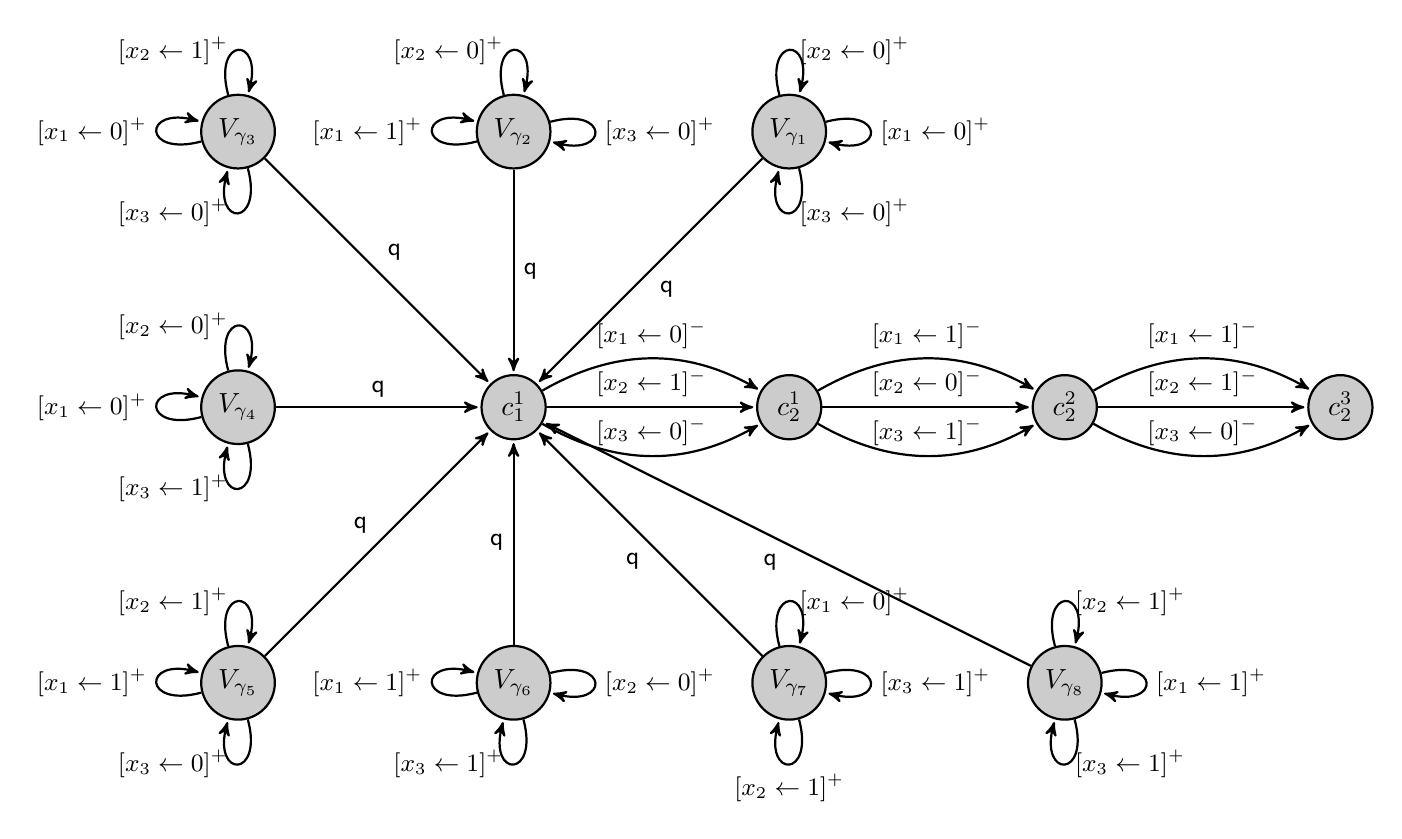
\begin{tikzpicture}[-,>=stealth',shorten >=1pt,auto,node distance=3.5cm,
  thick,main node/.style={circle,fill=black!20,draw}]

  
  \node[main node] (7) [] {$V_{\gamma_3}$};
  \node[main node] (8) [below of=7] {$V_{\gamma_4}$};
  \node[main node] (9) [below of=8] {$V_{\gamma_5}$};


  \node[main node] (1) [right of=8] {$c_1^1$};
  \node[main node] (2) [right of=1] {$c_2^1$};
  \node[main node] (3) [right of=2] {$c_2^2$};
  \node[main node] (4) [right of=3] {$c_2^3$};

  \node[main node] (5) [above of=2] {$V_{\gamma_1}$};
  \node[main node] (6) [above of=1] {$V_{\gamma_2}$};
  \node[main node] (10) [below of=1] {$V_{\gamma_6}$};
  \node[main node] (11) [below of=2] {$V_{\gamma_7}$};
  \node[main node] (12) [below of=3] {$V_{\gamma_8}$};


  \path[-> , every node/.style={font=\sffamily\small}]
    (5) edge [loop right, right] node  {$[x_1 \leftarrow 0]^+$}   (5)    
    (5) edge [loop above, right] node  {$[x_2 \leftarrow 0]^+$}  (5)    
    (5) edge [loop below, right] node  {$[x_3 \leftarrow 0]^+$}  (5)

    (5) edge [] node  {q}  (1)    
    

    (6) edge [loop left, left] node   {$[x_1 \leftarrow 1]^+$}   (6)    
    (6) edge [loop above, left] node  {$[x_2 \leftarrow 0]^+$}  (6)    
    (6) edge [loop right, right] node  {$[x_3 \leftarrow 0]^+$}  (6)

    (6) edge [] node  {q}  (1)    
         


    (7) edge [loop left, left] node   {$[x_1 \leftarrow 0]^+$}   (7)    
    (7) edge [loop above, left] node  {$[x_2 \leftarrow 1]^+$}  (7)    
    (7) edge [loop below, left] node  {$[x_3 \leftarrow 0]^+$}  (7)

    (7) edge [] node   {q}  (1)    
    


    (8) edge [loop left, left] node   {$[x_1 \leftarrow 0]^+$}   (8)    
    (8) edge [loop above, left] node  {$[x_2 \leftarrow 0]^+$}  (8)    
    (8) edge [loop below, left] node  {$[x_3 \leftarrow 1]^+$}  (8)

    (8) edge [] node  {q}  (1)    
    

    (9) edge [loop left, left] node   {$[x_1 \leftarrow 1]^+$}   (9)    
    (9) edge [loop above, left] node  {$[x_2 \leftarrow 1]^+$}  (9)    
    (9) edge [loop below, left] node  {$[x_3 \leftarrow 0]^+$}  (9)

    (9) edge [] node  {q}  (1)    

    
    (10) edge [loop left, left] node   {$[x_1 \leftarrow 1]^+$}   (10)    
    (10) edge [loop right, right] node  {$[x_2 \leftarrow 0]^+$}  (10)    
    (10) edge [loop below, left] node  {$[x_3 \leftarrow 1]^+$}  (10)

    (10) edge [] node   {q}  (1)    

    
    (11) edge [loop above, right] node    {$[x_1 \leftarrow 0]^+$}   (11)    
    (11) edge [loop below, below] node  {$[x_2 \leftarrow 1]^+$}  (11)    
    (11) edge [loop right, right] node  {$[x_3 \leftarrow 1]^+$}  (11)

    (11) edge [] node  {q}  (1)


    (12) edge [loop right, right] node  {$[x_1 \leftarrow 1]^+$}   (12)    
    (12) edge [loop above, right] node  {$[x_2 \leftarrow 1]^+$}  (12)    
    (12) edge [loop below, right] node  {$[x_3 \leftarrow 1]^+$}  (12)

    (12) edge [] node  {q}  (1)    
 

    (1) edge [bend left=30, above] node   {$[x_1 \leftarrow 0]^-$}  (2)
    (1) edge [bend left=0, above] node   {$[x_2 \leftarrow 1]^-$}  (2)
    (1) edge [bend right=30, above] node   {$[x_3 \leftarrow 0]^-$}  (2)
      

    (2) edge [bend left=30, above] node  {$[x_1 \leftarrow 1]^-$}  (3)
    (2) edge [bend left=0, above] node  {$[x_2 \leftarrow 0]^-$}  (3)
    (2) edge [bend right=30, above] node  {$[x_3 \leftarrow 1]^-$}  (3)
   

    (3) edge [bend left=30, above] node  {$[x_1 \leftarrow 1]^-$}  (4)
    (3) edge [bend left=0, above] node  {$[x_2 \leftarrow 1]^-$}  (4)
    (3) edge [bend right=30, above] node  {$[x_3 \leftarrow 0]^-$}  (4)
    
    ;

\end{tikzpicture}
\caption{Example of graph for $\Phi$}
\label{fig:sat_to_cfpq_graph_example}
\end{figure*}

\subsection{Improved reduction}

	
Firs step is to split variables into three group of the same size.
Suppose this splitting preserves the order.
So, we have a set of partial substitution. 
For our example:
\begin{align*}
\gamma_1^1 = \{x_1 \leftarrow 1 \} \\
\gamma_1^2 = \{x_1 \leftarrow 0 \} \\
\gamma_2^1 = \{x_2 \leftarrow 1 \} \\
\gamma_2^2 = \{x_2 \leftarrow 0 \} \\
\gamma_3^1 = \{x_3 \leftarrow 1 \} \\
\gamma_3^2 = \{x_3 \leftarrow 0 \} 
\end{align*}

By the same way we create vertices for partial subctitutions.



\begin{figure*}
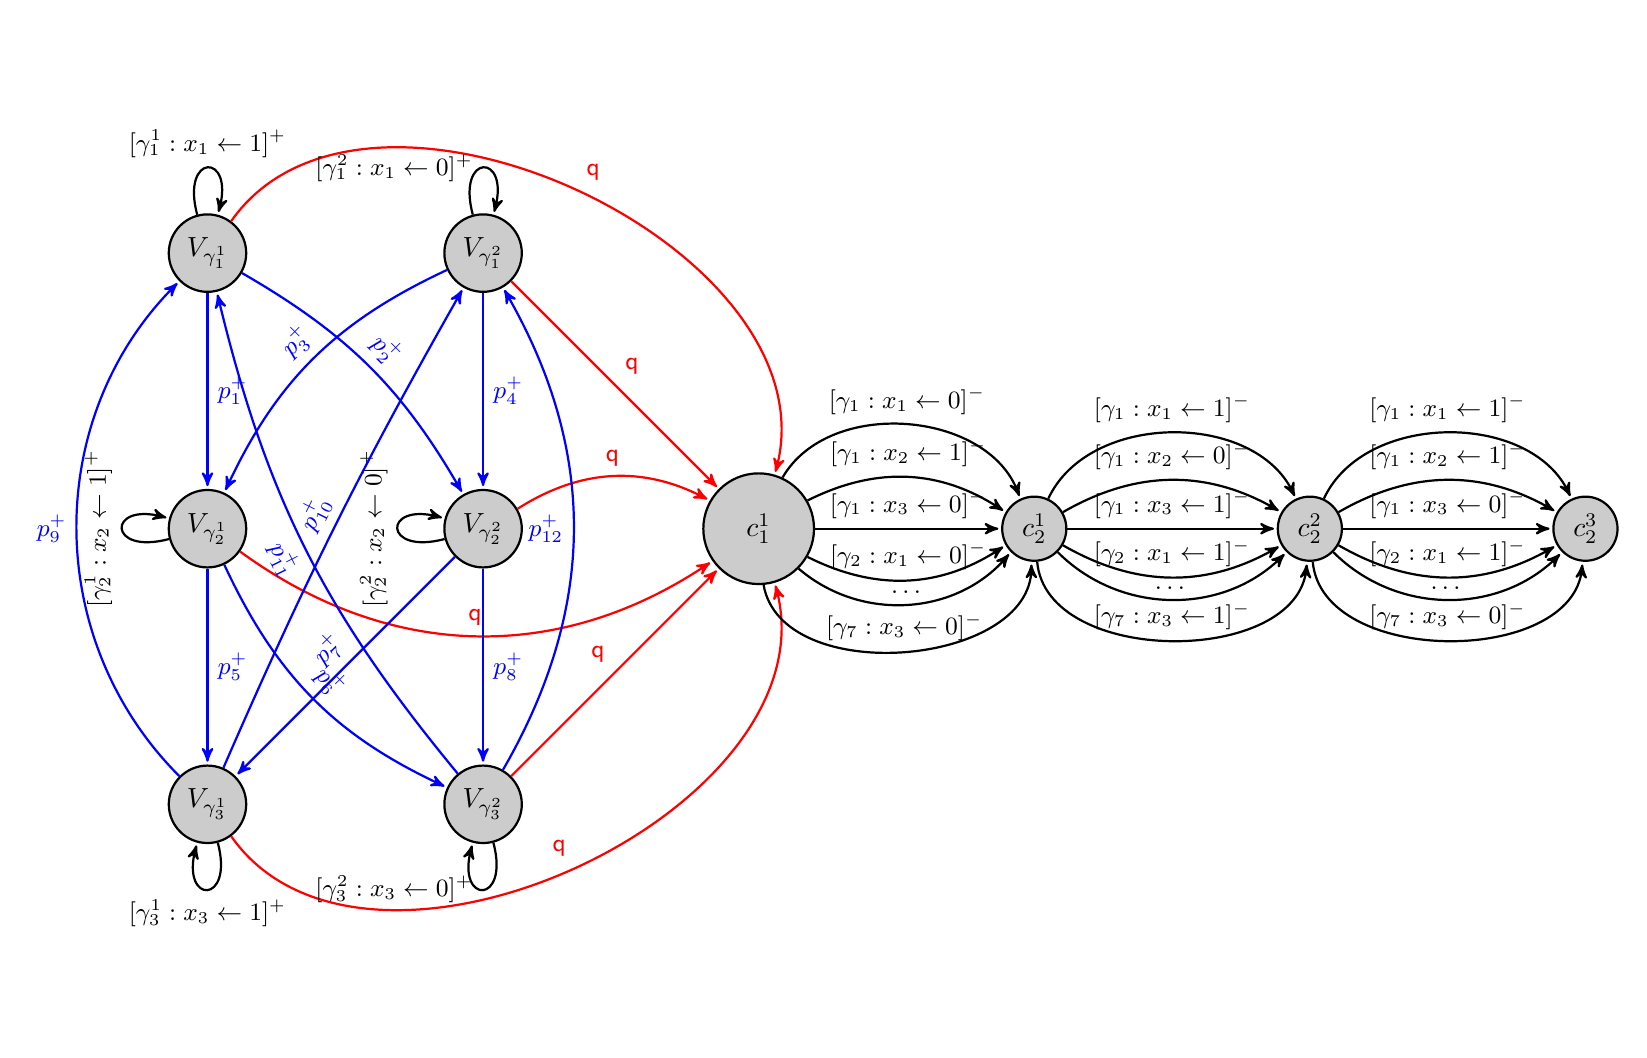
\begin{tikzpicture}[-,>=stealth',shorten >=1pt,auto,node distance=3.5cm,
  thick,main node/.style={circle,fill=black!20,draw}]

  
  \node[main node] (6) [] {$V_{\gamma_1^1}$};
  \node[main node] (7) [right of =6] {$V_{\gamma_1^2}$};
  \node[main node] (8) [below of=6] {$V_{\gamma_2^1}$};
  \node[main node] (9) [right of=8] {$V_{\gamma_2^2}$};
  \node[main node] (10) [below of=8] {$V_{\gamma_3^1}$};
  \node[main node] (11) [right of=10] {$V_{\gamma_3^2}$};
  


  \node[main node, minimum size = 40] (1) [right of=9] {$c_1^1$};
  \node[main node] (2) [right of=1] {$c_2^1$};
  \node[main node] (3) [right of=2] {$c_2^2$};
  \node[main node] (4) [right of=3] {$c_2^3$};

  
  \path[-> , every node/.style={font=\sffamily\small}]
    (6) edge [loop above, above] node  {$[\gamma_1^1: x_1 \leftarrow 1]^+$}   (6)    
    
    (6) edge [bend left = 80, color=red] node  {q}  (1)        
    (6) edge [color=blue] node  {$p_1^+$}  (8)
    (6) edge [color=blue, sloped, bend left=15] node  {$p_2^+$}  (9)                


    (7) edge [loop above, left] node  {$[\gamma_1^2: x_1 \leftarrow 0]^+$}   (7)    
    
    (7) edge [color=red] node {q}  (1)        
    (7) edge [color=blue, sloped, above, bend right=20] node  {$p_3^+$}  (8)
    (7) edge [color=blue] node  {$p_4^+$}  (9) 


    (8) edge [loop left, sloped, above] node  {$[\gamma_2^1: x_2 \leftarrow 1]^+$}   (8)    
    
    (8) edge [bend right=35, sloped, above, color=red] node  {q}  (1)        
    (8) edge [color=blue] node  {$p_5^+$}  (10)
    (8) edge [color=blue, sloped, bend right=20] node  {$p_6^+$}  (11) 

    (9) edge [loop left, above, sloped] node  {$[\gamma_2^2: x_2 \leftarrow 0]^+$}   (9)    
    
    (9) edge [color=red,bend left] node  {q}  (1)        
    (9) edge [color=blue, sloped, above] node  {$p_7^+$}  (10)
    (9) edge [color=blue] node  {$p_8^+$}  (11)     
    
    (10) edge [loop below, below] node  {$[\gamma_3^1: x_3 \leftarrow 1]^+$}   (10)    
    
    (10) edge [bend right=80,color=red] node  {q}  (1)        
    (10) edge [bend left=45, color=blue] node  {$p_9^+$}  (6)
    (10) edge [bend left=3, color=blue, above, sloped] node  {$p_{10}^+$}  (7) 
    
    (11) edge [loop below, left] node  {$[\gamma_3^2: x_3 \leftarrow 0]^+$}   (11)    
    
    (11) edge [color=red] node  {q}  (1) 
    (11) edge [bend left=13, color=blue, below, sloped] node  {$p_{11}^+$}  (6)
    (11) edge [bend right, color=blue] node  {$p_{12}^+$}  (7)


    (1) edge [bend left=65, above] node  {$[\gamma_1: x_1 \leftarrow 0]^-$}  (2)
    (1) edge [bend left=30, above] node  {$[\gamma_1: x_2 \leftarrow 1]^-$}  (2)
    (1) edge [bend right=0, above] node  {$[\gamma_1: x_3 \leftarrow 0]^-$}  (2)
    (1) edge [bend right=30, above] node  {$[\gamma_2: x_1 \leftarrow 0]^-$} (2)
    (1) edge [bend right=45, above] node  {$\dots$}                          (2)
    (1) edge [bend right=85, above] node  {$[\gamma_7: x_3 \leftarrow 0]^-$} (2)
    

    (2) edge [bend left=65, above] node  {$[\gamma_1: x_1 \leftarrow 1]^-$}  (3)
    (2) edge [bend left=30, above] node  {$[\gamma_1: x_2 \leftarrow 0]^-$}  (3)
    (2) edge [bend right=0, above] node  {$[\gamma_1: x_3 \leftarrow 1]^-$}  (3)
    (2) edge [bend right=30, above] node  {$[\gamma_2: x_1 \leftarrow 1]^-$} (3)
    (2) edge [bend right=45, above] node  {$\dots$}                          (3)
    (2) edge [bend right=85, above] node  {$[\gamma_7: x_3 \leftarrow 1]^-$} (3)

    (3) edge [bend left=65, above] node  {$[\gamma_1: x_1 \leftarrow 1]^-$}  (4)
    (3) edge [bend left=30, above] node  {$[\gamma_1: x_2 \leftarrow 1]^-$}  (4)
    (3) edge [bend right=0, above] node  {$[\gamma_1: x_3 \leftarrow 0]^-$}  (4)
    (3) edge [bend right=30, above] node  {$[\gamma_2: x_1 \leftarrow 1]^-$} (4)
    (3) edge [bend right=45, above] node  {$\dots$}                          (4)
    (3) edge [bend right=85, above] node  {$[\gamma_7: x_3 \leftarrow 0]^-$} (4)
    
    ;

\end{tikzpicture}
\caption{Example of graph for $\Phi$}
\label{fig:sat_to_cfpq_graph_example}
\end{figure*}
\documentclass[12pt]{article}  % standard LaTeX, 12 point type
\usepackage{amsfonts,latexsym}
\usepackage{amsthm}
\usepackage{amssymb}
\usepackage[utf8x]{inputenc} % Кодировка
\usepackage[english]{babel} % Многоязычность
\usepackage{amsmath}
\usepackage{tikz}
\usetikzlibrary{automata,positioning}

\usepackage{algpseudocode}
\usepackage{algorithm}
\usepackage{caption}
\usepackage{algorithmicx}


\newtheorem{theorem}{Theorem}[section]
\newtheorem{proposition}[theorem]{Proposition}
\newtheorem{lemma}[theorem]{Lemma}
\newtheorem{corollary}[theorem]{Corollary}
\newtheorem{conjecture}[theorem]{Conjecture}

\theoremstyle{definition}
\newtheorem{definition}{Определение}[section]
\newtheorem{example}{Example}[section]

% unnumbered environments:

\theoremstyle{remark}
\newtheorem*{remark}{Remark}
\newtheorem*{notation}{Notation}
\newtheorem*{note}{Note}

\setlength{\parskip}{5pt plus 2pt minus 1pt}
%\setlength{\parindent}{0pt}

\usepackage{color}
\usepackage{listings}
\usepackage{caption}
\usepackage{graphicx}
\usepackage{ucs}

\newcommand{\tab}[1][0.3cm]{\ensuremath{\hspace*{#1}}}
% A generalized view on parsing and translation
% http://dl.acm.org/citation.cfm?id=2206331
\title{Arbirary CFPQ to Dyck language constrained querying}
% Context-free path querying ...
\author{Semyon Grigorev
\\
       {Saint Petersburg State University}\\
       {7/9 Universitetskaya nab.}\\
       {St. Petersburg, 199034, Russia}\\
       semen.grigorev@jetbrains.com, rsdpisuy@gmail.com
       }
\date{}

\begin{document}

\algtext*{EndWhile}% Remove "end while" text
\algtext*{EndIf}% Remove "end if" text
\algtext*{EndFor}% Remove "end for" text
\algtext*{EndFunction}% Remove "end function" text

\maketitle

This reduction is inspired by the construction described in~\cite{OptimalDLR}.

Consider a context-free grammar $\mathcal{G}=(\Sigma, N, P, S)$ in BNF where $\Sigma$ is a terminal alphabet, $N$ is 
a nonterminal alphabet, $P$ is a set of productions, $S \in N$ is a start nonterminal.
Also we denote a directed labeled graph by $G=(V,E,L)$ where $E \subseteq V \times L \times V$ and $L \subseteq \Sigma$. 

We should construct new input graph $G'$ and new grammar $\mathcal{G'}$ such that $\mathcal{G'}$ specifies a Dyck language and there is a simple mapping from $\text{CFPQ}(\mathcal{G'}, G')$ to $\text{CFPQ}(\mathcal{G}, G)$.
Step-by-step example with description is provided below.
 
Let the input grammar is 
\begin{align*}
S & \rightarrow a \ S \ b \ | \ a \ C \ b 
\\
C & \rightarrow c \ | \ C \ c
\end{align*}

Let the input graph is
\\
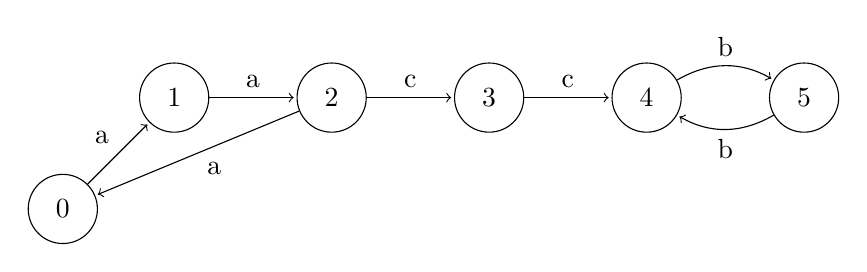
\begin{tikzpicture}[shorten >=1pt,node distance=2cm,on grid,auto] 
   \node[state] (q_0)   {$0$}; 
   \node[state] (q_1) [above right=of q_0] {$1$}; 
   \node[state] (q_2) [right=of q_1] {$2$}; 
   \node[state] (q_3) [right=of q_2] {$3$};
   \node[state] (q_4) [right=of q_3] {$4$};
   \node[state] (q_5) [right=of q_4] {$5$};
    \path[->] 
    (q_0) edge  node {a} (q_1)          
    (q_1) edge  node {a} (q_2)
    (q_2) edge  node {a} (q_0)
    (q_2) edge  node {c} (q_3)
    (q_3) edge  node {c} (q_4)
    (q_4) edge[bend left, above]  node {b} (q_5)
    (q_5) edge[bend left, below]  node {b} (q_4);
\end{tikzpicture}

\begin{enumerate}
\item Let $\Sigma_{()} =\{ t_( , t_)  | t \in \Sigma \}$.
\item Let $N_{()} = \{ N_( , N_) | N \in N  \}$.
\item Let $M_{\mathcal{G}} = (V_{\mathcal{G}}, E_{\mathcal{G}}, L_{\mathcal{G}})$ is a directed 
labeled graph, where $L_{\mathcal{G}} \subseteq (\Sigma_{()} \cup N_{()})$.
This graph is created the same manner as described in~\cite{OptimalDLR} but we do not require the grammar be in CNF.
Let $x \in V_{\mathcal{G}}$ and $y \in V_{\mathcal{G}}$ is ``start'' and ``final'' vertices respectively. 
This graph may be treated as a finite automaton, so it can be minimized and we can compute an $\varepsilon$-closure if the input grammar contains $\varepsilon$ productions.
The graph $M_{\mathcal{G}}$ for our example is:
\\
\includegraphics[width=.7\textwidth]{dot/grammar_1.pdf}


The minimized graph:
\\
\includegraphics[width=.7\textwidth]{dot/grammar_min.pdf}


\item For each $v \in V$ create $M_{\mathcal{G}}^v$: unique instance of $M_{\mathcal{G}}$.
\item New graph $G^{'}$ is a graph $G$ where each label $t$ is replaced with $t_{)}^i$ and some additional edges are created:
\begin{itemize}
\item Add an edge $(v', S_(, v)$ for each $v \in V$. 
\item And the respective $M_{\mathcal{G}}^v$ for each $v \in V$:
  \begin{itemize}
    \item reattach all edges outgoing from $x^v$ (``start'' vertex of $M_{\mathcal{G}}^v$) to $v$;
    \item reattach all edges incoming to $y^v$ (``final'' vertex of $M_{\mathcal{G}}^v$) to $v$.    
  \end{itemize}
  New input graph is ready:
  
  \includegraphics[width=.9\textwidth]{dot/input_new_min.pdf}
\end{itemize}

\item New grammar $\mathcal{G'}=(\Sigma^{'}, N', P', S')$ where $\Sigma^{'} = \Sigma_{()} \cup N_{()}$, $N' = \{ S' \}$, $P' = \{ S' \rightarrow b_( \ S' \ b_); S' \rightarrow b_( \ b_) \ | \ b_(, b_{)} \in \Sigma^{'} \} \cup \{ S' \rightarrow S' \ S' \}$ is a set of productions, $S' \in N'$ is a start nonterminal.
\end{enumerate}

Now, if $\text{CFPQ}(\mathcal{G'}, G')$ contains a pair $(u'_0, v')$ such that $e=(u'_0, S_( , u'_1) \in E'$ is an extension edge (step 5, first subitem), then  $(u'_1, v') \in \text{CFPQ}(\mathcal{G}, G)$.
In our example, we can find the following path: $7 \xrightarrow{S_(} 1 \xrightarrow{S_)} 22 \xrightarrow{b_(} 25 \xrightarrow{C_(} 26 \xrightarrow{a_(} 1   
\xrightarrow{a_)} 2 \xrightarrow{C_)} 33 \xrightarrow{C_(} 34 \xrightarrow{c_(} 2  \xrightarrow{c_)} 3 \xrightarrow{C_)} 43 \xrightarrow{c_(} 3 \xrightarrow{c_)} 4 \xrightarrow{b_)} 5$. 
Edge $7 \xrightarrow{S_(} 1$ is the extension, so (1,5) should be in $\text{CFPQ}(\mathcal{G}, G)$ and it is true.


\section{Modified algorithm}

\begin{algorithm}[!ht]
\begin{algorithmic}[1]
\caption{Digraph flat exact paths}
\label{parsing}
\Function{Digraph-flat-exact-paths}{$G$}
  \State{$\{{D_k}^{(-1)}, {D_k}^{(0)}, {D_k}^{(+1)} \} \gets$ \Call{Init-Adjacency-Matrices}{$G$}}
  \State{$M_1 \gets$ \Call{AGMY-Code-then-Sum}{${D_1}^{(-1)}, {D_1}^{(0)}, {D_1}^{(+1)}$}}
  \State{$\dots$}
  \State{$M_k \gets$ \Call{AGMY-Code-then-Sum}{${D_k}^{(-1)}, {D_k}^{(0)}, {D_k}^{(+1)}$}}
  \State{$n \gets |V|$}
  \For{$l \in [2 \dots \lceil \text{log} \ n \rceil + 1]$} \Comment{Upper bound should be analized carefully}
     \State{$M' \gets $ \Call{Markup-Minus-One-Edges}{$M_1$}} \Comment{AGMY, mark $-1$ edges}     
     \State{$M_1 \gets M' \times M_1$}  \Comment{AGMY, non-Dyck 0 edges are detectable}
     \State{$\dots$} \Comment{Do for all $M_i$}
     \State{$M_k \gets M_k \times M_k$}
     \State{Remove $\pm 1$ edges from all $M_i$}
     \State{$M_1 \gets$ \Call{Normalize-and-Divide-by-2}{$M_1$}}
     \State{$\dots$}
     \State{$M_k \gets$ \Call{Normalize-and-Divide-by-2}{$M_k$}}
     \State{$Z \gets$ \Call{Get-Zero-Edges}{$M_1$}}
     \State{$Z \gets Z + $ \Call{Get-Zero-Edges}{$M_2$}}
     \State{$\dots$}
     \State{$Z \gets Z + $ \Call{Get-Zero-Edges}{$M_k$}}
     \State{$M_1 \gets Z \times M_1 \times Z$}  \Comment{AGMY, extend $\pm 1$  and 0 edges for all $M_i$}
     \State{$\dots$}
     \State{$M_k \gets Z \times M_k \times Z$}
  \EndFor
\EndFunction
\end{algorithmic}
\end{algorithm}


\begin{thebibliography}{9}

\bibitem{OptimalDLR}
Krishnendu Chatterjee, Bhavya Choudhary, and Andreas Pavlogiannis. 
2017. 
\emph{Optimal Dyck reachability for data-dependence and alias analysis.}
Proc. ACM Program. Lang. 2, POPL, Article 30 (December 2017), 30 pages. DOI: 
https://doi.org/10.1145/3158118


%\bibitem{ParsingWithPictures}
%  Keshav Pingali, and Gianfranco Bilardi. 
%  \emph{A Graphical Model for Context-Free Grammar Parsing.}
%   International Conference on Compiler Construction. Springer, Berlin, Heidelberg, 2015.


\end{thebibliography}


\end{document}
%\section{two brs}

Let the input grammar is 
\begin{align*}
S & \rightarrow a \ S \ b \ 
\\
S & \rightarrow c \ S \ d \
\\
S & \rightarrow a \ b
\\
S & \rightarrow c \ d
\end{align*}

The input grammar in CNF is 
\begin{align*}
S   & \rightarrow A \ S_1
\\
S_1 & \rightarrow S \ B
\\
S   & \rightarrow C \ S_2
\\
S_2 & \rightarrow S \ D
\\
S   & \rightarrow C \ D
\\
S   & \rightarrow A \ B
\\
C   & \rightarrow c
\\
D   & \rightarrow d
\\
A   & \rightarrow a
\\
B   & \rightarrow b
\end{align*}


Let the input graph is:
\\
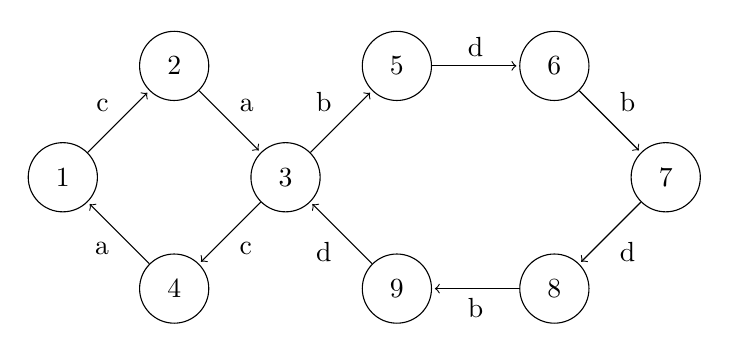
\begin{tikzpicture}[shorten >=1pt,node distance=2cm,on grid,auto] 
   \node[state] (q_1)   {$1$}; 
   \node[state] (q_2) [above right=of q_1] {$2$}; 
   \node[state] (q_3) [below right=of q_2] {$3$}; 
   \node[state] (q_4) [below right=of q_1] {$4$};
   \node[state] (q_5) [above right=of q_3]  {$5$}; 
   \node[state] (q_6) [right=of q_5] {$6$}; 
   \node[state] (q_7) [below right=of q_6] {$7$}; 
   \node[state] (q_9) [below right=of q_3] {$9$};
   \node[state] (q_8) [right=of q_9] {$8$};

    \path[->] 
    (q_1) edge  node {c} (q_2)          
    (q_2) edge  node {a} (q_3)
    (q_3) edge  node {c} (q_4)
    (q_4) edge  node {a} (q_1)

    (q_3) edge  node {b} (q_5)          
    (q_5) edge  node {d} (q_6)
    (q_6) edge  node {b} (q_7)
    (q_7) edge  node {d} (q_8)
    (q_8) edge  node {b} (q_9)
    (q_9) edge  node {d} (q_3)
    
    ;
\end{tikzpicture}




%\bibliographystyle{abbrv}
\bibliographystyle{ACM-Reference-Format}
\bibliography{SAT_to_CFPQ}



\end{document}